\section{Finite-Element-Methode 3D}

\subsection{3D elektrostatisches Randwertproblem}
\begin{minipage}[c]{0.36\columnwidth}
    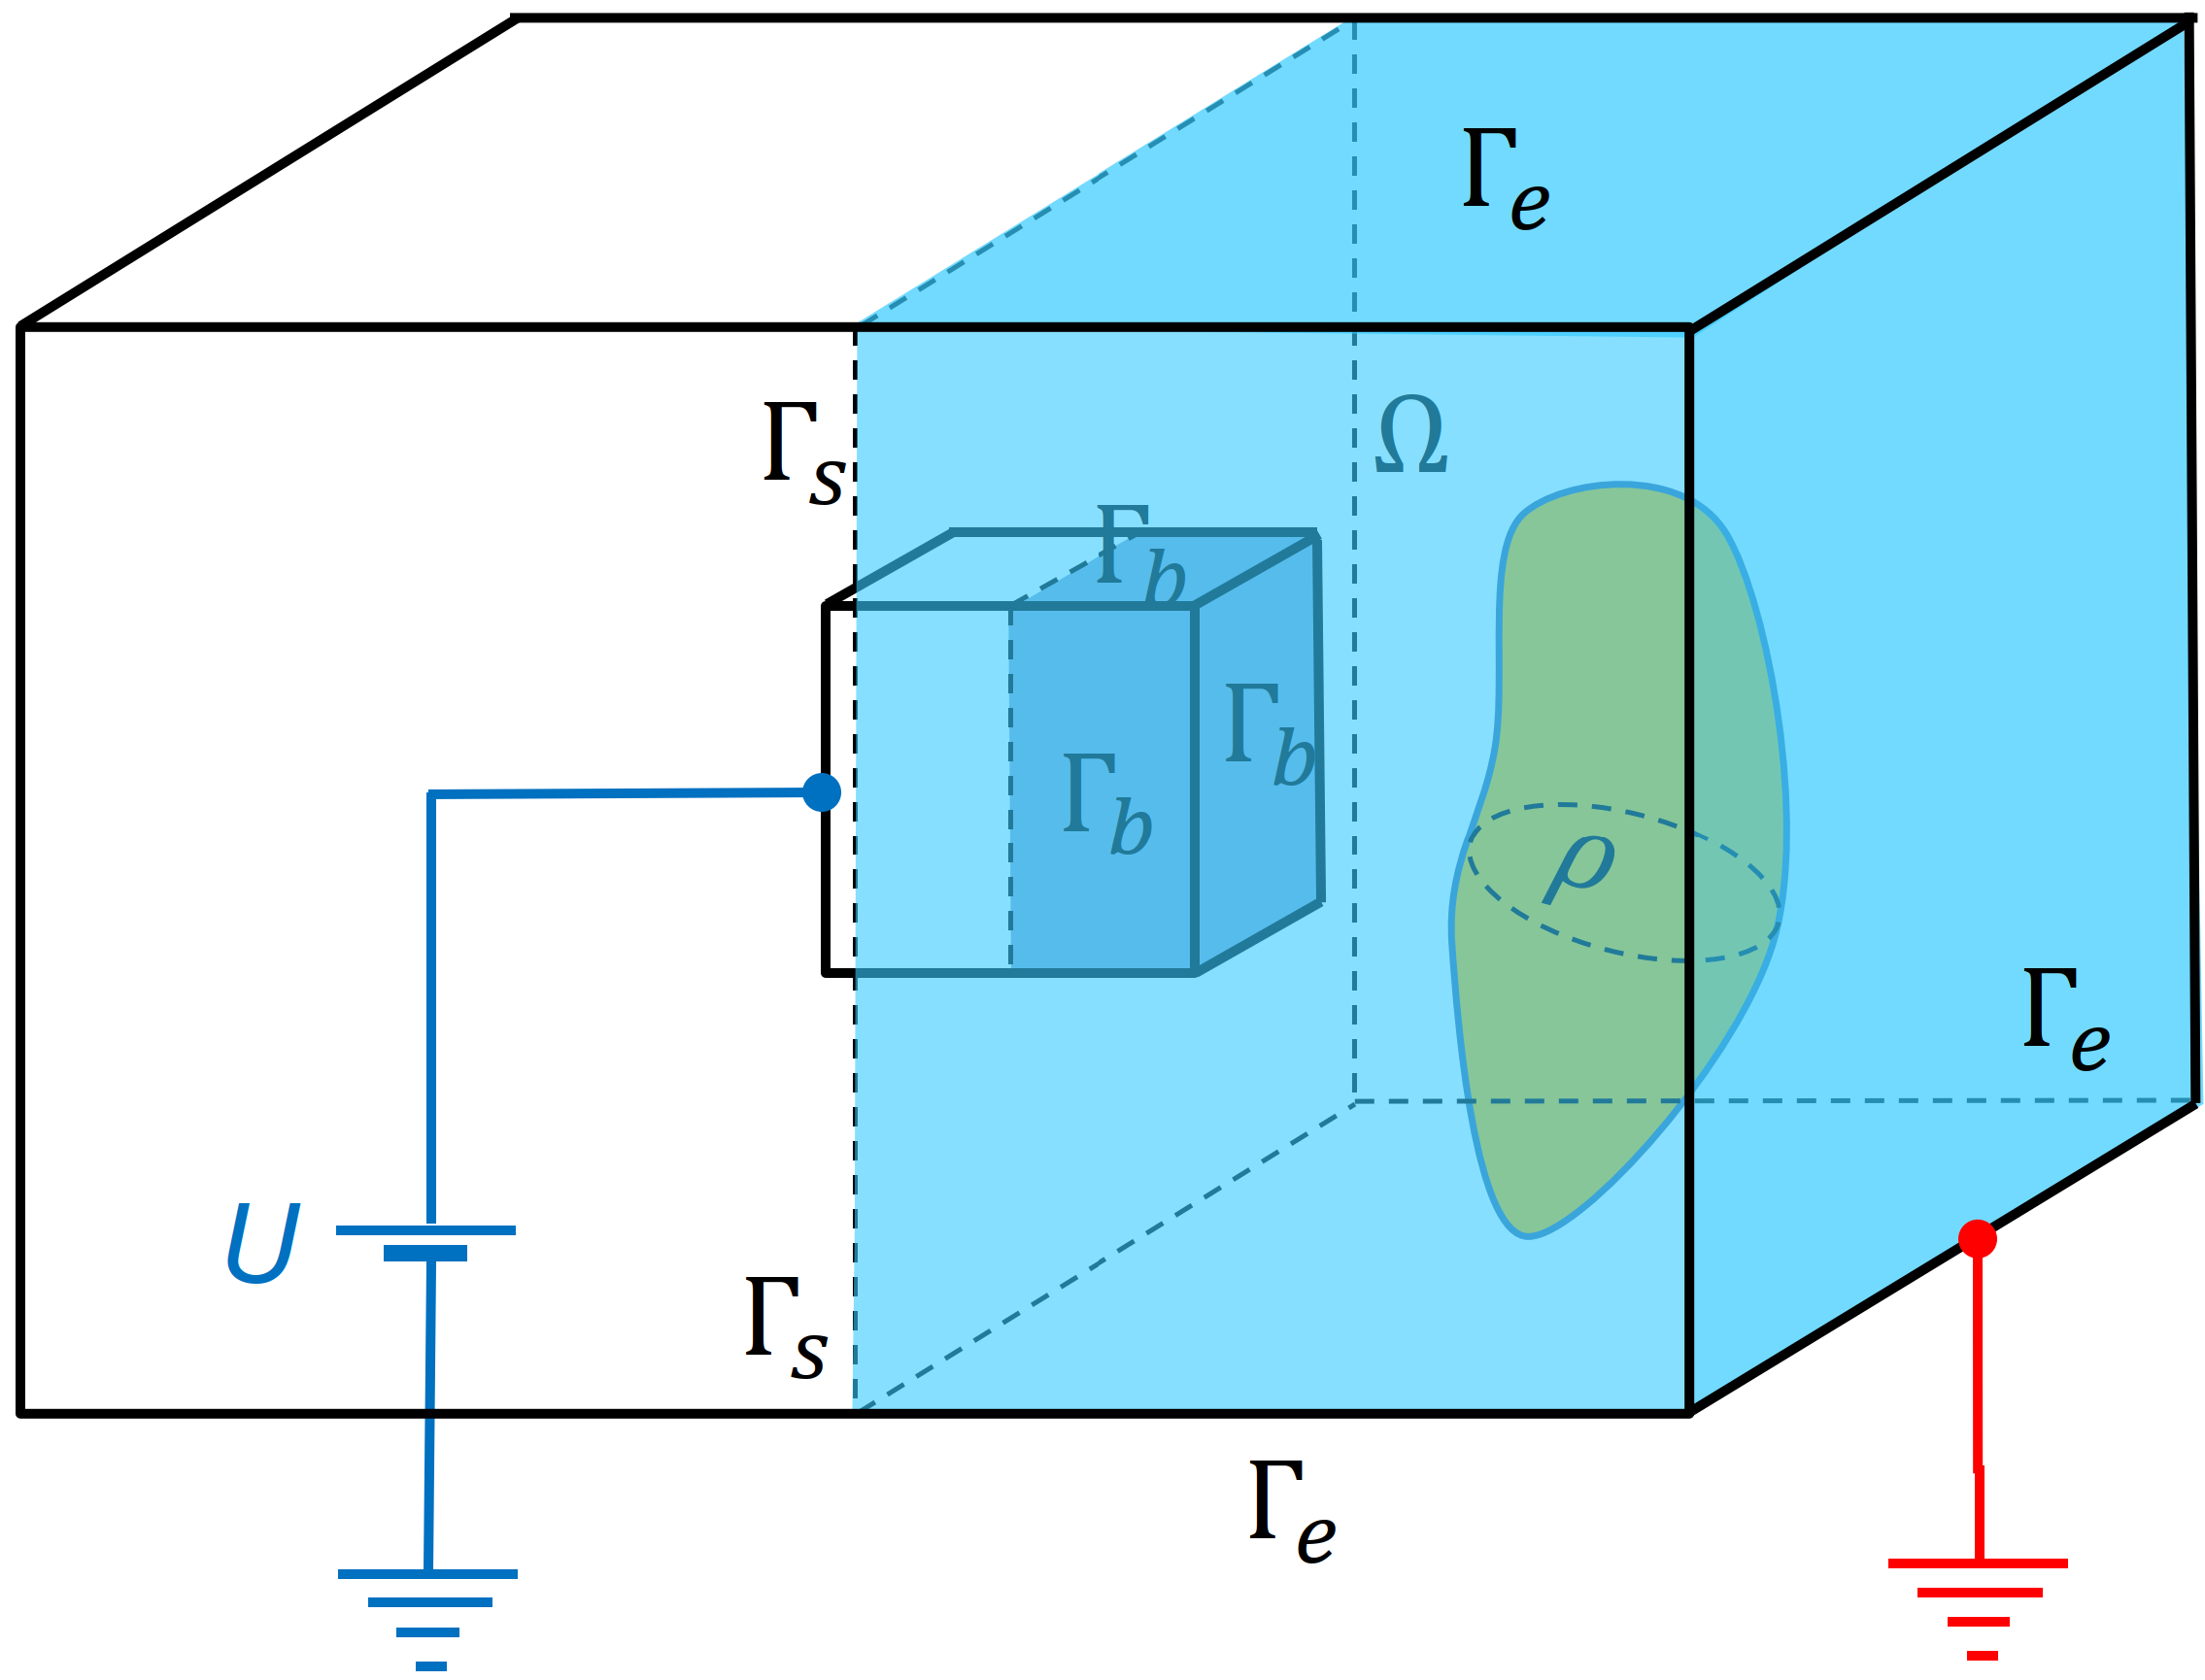
\includegraphics[align=t, width=0.85\columnwidth]{images/V7B1.png}
\end{minipage}
\hfill
\begin{minipage}[c]{0.60\columnwidth}
    
     
    $\underset{(C)}{\operatorname*{\oint}} \vec{E} \cdot\vec{dl} 
    = \underset{(C_1)}{\operatorname*\int_{P_1}^{P_2}} \vec{E} \cdot \,\vec{dl} 
    - \underset{(C_2)}{\operatorname*\int_{P_1}^{P_2}} \vec{E} \cdot \,\vec{dl} 
    = 0$\\
    $\underset{(C_1)}{\operatorname*\int_{P_1}^{P_2}} \vec{E} \cdot \,\vec{dl} 
    = \underset{(C_2)}{\operatorname*\int_{P_1}^{P_2}} \vec{E} \cdot \,\vec{dl}$
\end{minipage}

\begin{tabular}{lll}
    $\left[\rho\right]$ &=& elektrische Raumladungsdichte $\frac{C}{m^3} = \frac{A \cdot s}{m^3}$\\
    $\left[\varepsilon\right]$ &=& elektrische Permittivität $\frac{C}{V \cdot m} = \frac{A \cdot s}{V \cdot m}$\\
    $\left[\varphi\right]$ &=& (unbekannte) elektrische Potentialverteilung $\frac{V}{m}$\\
    $\left[\Omega\right]$ &=& Rechengebit $\frac{}{}$\\
    $\left[\Gamma_e\right]$ &=& geerdeter Rand $\frac{}{}$\\
    $\left[E\right]$ &=& elektrische Feldstärke $\frac{V}{m}$\\
    $\left[Q\right]$ &=& elektrische Ladung $C = A \cdot s$\\
    $\left[A\right]$ &=& Oberfläche des Volumen $m^2$
\end{tabular}